\chapter{Tier 1: deterministic investment appraisal}\label{chap:tier1}
\section{Problem analysis}\label{sec:problem1}
Given the paths in Chapter~\ref{chap:common}, we choose equipment capacity
and daily use. Electricity can be sold, stored, converted to hydrogen or
left unused. The objective is equivalent annual profit gain relative to
no investment under the same operating rules, after capital, fixed operation
and renewal costs.

Open choices concern displacement of electricity sales, hydrogen offtake
and value, equipment cost scope, discount rate and battery chronology.
We specify these below and test the choices that change the investment.

\section{Assumptions and research}\label{sec:research1}
\subsection{Tier-specific assumptions}
Investment is once at the start, in whole reference modules. Electrolysers
can be off or run at 20--100\% of online module power. Hydrogen is sold
directly, with no storage or reconversion. Its netback (receipts after
non-electricity variable costs) is assumed to equal a rebased support value.
The 10 t/day buyer limit and 5\% real discount rate are analytical assumptions.

We distinguish \emph{policy A}, which allocates generation freely by economic
value, and \emph{policy B}, which first sells \(\min(G_t,D_t)\) each day.
B sells even at negative prices. Each has its own zero-investment comparator.
Battery energy is balanced over the sample, with at most one usable window
per day; fixed nonzero batteries are also checked chronologically.
This follows the simplified Tier 1 time treatment \cite{brief,teacher}.

\subsection{Research objectives and parameter selection}
Research establishes market boundaries, equipment scale and performance,
cost scope and financial comparability (Table~\ref{tab:research}). The battery
module is a research reference; the brief specifies its two-hour duration.

The brief's \gbp 9.50/kg hydrogen benchmark has no explicit price base.
We convert the published \gbp 175/MWh in 2012 pounds using 39.4 kWh/kg
and the 2020/2012 consumer-price-index ratio. The resulting netback assumes
no further non-power deduction. Electrolyser capital uses the midpoint of
the published US\$2,000--2,600/kW installed range. These reference estimates
motivate the hydrogen-value, offtake, capital and discount sensitivities.

\begin{table}[H]
\centering\small
\caption{Technical and financial research used in Tier 1. Costs are in 2020 pounds.}
\label{tab:research}
\begin{tabularx}{\linewidth}{@{}P{.17\linewidth}P{.43\linewidth}Y@{}}
\toprule
Research objective & Selected input & Source and evidence scope \\
\midrule
Battery performance and scale &
1.5 MW / 3 MWh module; 20--80\% state of charge; 90\% round-trip efficiency;
15-year life & Brief and Danish Energy Agency technology catalogue; reference
equipment, not a supplier offer \cite{brief,dea}. \\
Battery cost &
\gbp 256,235/MWh capital; \gbp 14,862/MW-year fixed operation &
Brief's EUR 288,000/MWh converted with 2020 exchange rate; 2.9\% annual
maintenance convention \cite{basis}. \\
Electrolysis operation &
20 MW modules; 20--100\% online load; 55.9 kWh/kg; 30-year life &
Brief technical reference; life and renewal assumptions from UK production
cost estimates \cite{brief,beis}. \\
Financial comparability &
Monthly inflation adjustment; 5\% real discount; zero terminal value &
Public inflation/exchange-rate series; discount sensitivity; zero residual assumed \cite{cpi,basis}. \\
\bottomrule
\end{tabularx}
\end{table}
\begin{table}[H]\ContinuedFloat
\centering\small
\caption[]{Technical and financial research (continued).}
\begin{tabularx}{\linewidth}{@{}P{.17\linewidth}P{.43\linewidth}Y@{}}
\toprule
Research objective & Selected input & Source and evidence scope \\
\midrule
Electrolyser costs &
\gbp\Capital m per module; \gbp 0.517m/year fixed cost;
\gbp 9.792m stack renewal in years 11 and 22 &
Installed-cost survey midpoint; separate absolute UK fixed and stack
proxies, rather than applying an old stack percentage to new capital \cite{iea,beis}. \\
Hydrogen outlet and value &
Direct sale; \gbp\Netback/kg netback; 10,000 kg/day &
UK hydrogen support reference rebased to 2020; realised-netback and buyer-cap
scenarios, not a verified market contract \cite{har,basis}. \\
\bottomrule
\end{tabularx}
\end{table}

\section{Mathematical model}\label{sec:model1}
\begin{table}[H]
\centering\small
\caption{Tier 1 notation, additional to Chapter~\ref{chap:common}.}
\begin{tabularx}{\linewidth}{@{}lY r@{}}
\toprule
Symbol & Meaning & Unit or domain \\
\midrule
\(b,n\) & Installed battery and electrolyser modules & \(\mathbb Z_{\ge0}\) \\
\(z_t\) & Online electrolyser modules on day \(t\) & \(\mathbb Z_{\ge0}\) \\
\(q_t,c_t,r_t\) & Direct sale, battery charge and discharge & MWh \\
\(h_t,u_t\) & Electrolysis electricity input and unused generation & MWh \\
\(v,L,\kappa\) & Hydrogen netback, daily buyer cap and electricity per kg & \gbp/kg; kg/day; MWh/kg \\
\(E_B,\eta\) & Usable battery module energy and one-way efficiency & MWh; dimensionless \\
\(E_H^{\min},E_H^{\max}\) & Online module's daily input limits & MWh \\
\(a_B,a_H\) & Equivalent annual costs per installed module & \gbp/year \\
\bottomrule
\end{tabularx}
\end{table}
Here \(\kappa=0.0559\), \(E_B=1.8\), \(\eta=\sqrt{0.90}\) and
\((E_H^{\min},E_H^{\max})=(96,480)\), in the units above. Let \(x\)
collect the installed capacities and daily decisions. The annual profit
before subtracting the constant no-investment comparator is
\begin{equation}
\max_x\;\Pi(x)=\frac{1}{Y}\sum_{t\in\mathcal T}
 \left[p_t(q_t+r_t)+\frac{v h_t}{\kappa}\right]-a_Bb-a_Hn.
\label{eq:profit}
\end{equation}
The feasible set is defined by
\begin{subequations}\label{eq:constraints}
\begin{align}
q_t+c_t+h_t+u_t&=G_t,&q_t+r_t&\le D_t,\label{eq:flow}\\
c_t&\le E_Bb/\eta,&r_t&\le\eta E_Bb,\label{eq:window}\\
\sum_t r_t&=\eta^2\sum_t c_t,\label{eq:pool}\\
E_H^{\min}z_t\le h_t&\le E_H^{\max}z_t,&h_t/\kappa&\le L,&z_t&\le n,\label{eq:hydrogen}\\
q_t,c_t,r_t,h_t,u_t&\ge0,&b,n,z_t&\in\mathbb Z_{\ge0}.\label{eq:domains}
\end{align}
\end{subequations}
All day-indexed constraints hold for every \(t\in\mathcal T\).
Equation~\eqref{eq:flow} allocates generation and limits total electricity
sales. Equations~\eqref{eq:window}--\eqref{eq:pool} link battery throughput
to installed capacity and impose the round-trip loss. Equation~\eqref{eq:hydrogen}
enforces online loading, daily hydrogen acceptance and installed capacity;
zero online modules allow shutdown. Equation~\eqref{eq:domains} gives
nonnegativity and integrality. Policy B adds \(q_t=\min(G_t,D_t)\).

For asset \(j\in\{B,H\}\), equivalent annual cost is
\begin{equation}
a_j=F_j+\frac{i}{1-(1+i)^{-N_j}}
 \left(K_j+\sum_{k\in\mathcal R_j}\frac{C_{jk}}{(1+i)^k}\right),
\label{eq:annualcost}
\end{equation}
where \(F_j\) is fixed annual operation, \(K_j\) initial capital including
commissioning, \(N_j\) life, \(i\) discount rate and \(C_{jk}\) renewal cost
in the years \(\mathcal R_j\). At \(i=0\), the capital-recovery factor is
\(1/N_j\). The reported gain is \(\Pi(x)-\Pi(x_0)\), where \(x_0\)
is the same-policy zero-investment solution. Subtracting this constant
leaves the optimum unchanged.

\section{Results and analysis}\label{sec:results1}
\subsection{Capacity and historical performance}
Table~\ref{tab:annual}(a) compares the allowed asset sets in the 2023
stress year. For the six complete years 2020--25, we optimise one common
size: both policies select 20 MW electrolysis and no batteries.
Panel (b) replays that fixed size annually, including production and surplus
capture. The 2026 partial year is archived separately. The detailed
comparisons use 2023, the complete year with the least surplus.
\begin{table}[H]
\centering\small
\caption{Investment and operating results: capacities in MW, hydrogen in t/year, gains in \gbp m/year against each policy's zero investment. Panel (b) capture is identical in A and B.}
\label{tab:annual}
\textit{(a) 2023: asset-set optimisation and fixed-capacity comparison}\par\vspace{2pt}
\begin{tabular}{@{}l r r r r r r@{}}
\toprule
 & \multicolumn{3}{c}{Policy A} & \multicolumn{3}{c}{Policy B} \\
\cmidrule(lr){2-4}\cmidrule(l){5-7}
Allowed investment & Battery & Electrolyser & Gain & Battery & Electrolyser & Gain \\
\midrule
No investment & 0 & 0 & 0.00 & 0 & 0 & 0.00 \\
Battery only & 0 & 0 & 0.00 & 0 & 0 & 0.00 \\
Electrolyser only & 0 & 20 & 8.57 & 0 & 0 & 0.00 \\
Joint choice & 0 & 20 & 8.57 & 0 & 0 & 0.00 \\
Fixed 20 MW & 0 & 20 & 8.57 & 0 & 20 & \minus{1.07} \\
\bottomrule
\end{tabular}
\par\vspace{5pt}
\textit{(b) Fixed 20 MW on every complete year}\par\vspace{2pt}
\begin{tabular}{@{}l r r r r r r r@{}}
\toprule
Year & \shortstack{Surplus\\days} & \shortstack{Surplus\\(GWh)} & \shortstack{Capture\\(GWh)} & H$_2$ A & H$_2$ B & Gain A & Gain B \\
\midrule
2020 & 92 & 2067 & 43.9 & 3143 & 786 & 16.78 & 3.12 \\
2021 & 43 & 911 & 20.6 & 2301 & 369 & 6.29 & \minus{0.13} \\
2022 & 154 & 4240 & 73.9 & 2009 & 1322 & 8.91 & 7.31 \\
2023 & 29 & 550 & 13.9 & 3074 & 249 & 8.57 & \minus{1.07} \\
2024 & 30 & 1229 & 14.4 & 3134 & 258 & 11.95 & \minus{1.00} \\
2025 & 112 & 4660 & 53.7 & 3126 & 960 & 13.17 & 4.48 \\
Mean & -- & 2276 & 36.7 & 2798 & 657 & 10.94 & 2.12 \\
\bottomrule
\end{tabular}
\end{table}

The positive B mean includes three losing years. Its freely chosen 2023
investment is zero, whereas a fixed 20 MW asset loses money. A sale-first
rule on that asset reproduces B and makes \gbp 9.64m/year less than A's
optimised dispatch: A produces more hydrogen by diverting saleable power,
while both capture the same surplus. Battery-only optimisation chooses zero
in both policies; hydrogen-only and joint choices coincide.

\subsection{Energy attribution and contract sensitivity}
In 2023 the electrolyser takes \Hinput~GWh: \Capture~GWh from physical
surplus and \Displaced~GWh diverted from direct sale. Thus only
\CaptureShare\% of its input is surplus capture, equivalent to
\SurplusShare\% of that year's \Surplus~GWh surplus. The 29 surplus days
each use the full 0.48 GWh module input. The 10 t/day buyer cap can accept
at most 0.559 GWh/day of electrolysis input, limiting pure surplus capture
to \PhysicalCap~GWh even with larger equipment.

Fuel aggregates do not identify which generator supplied electrolysis.
Under surplus-first attribution, define captured energy
\(C_t=\min(h_t,S_t)\) and wind-plus-solar generation \(R_t\). Its
contribution \(W_t\) to capture satisfies
\begin{equation}
\max\{0,C_t-(G_t-R_t)\}\le W_t\le\min\{C_t,R_t\}.
\end{equation}
The annual interval is 0--\Capture~GWh; adding biomass and run-of-river
hydro to the renewable category leaves these bounds unchanged.

\begin{figure}[H]
\centering
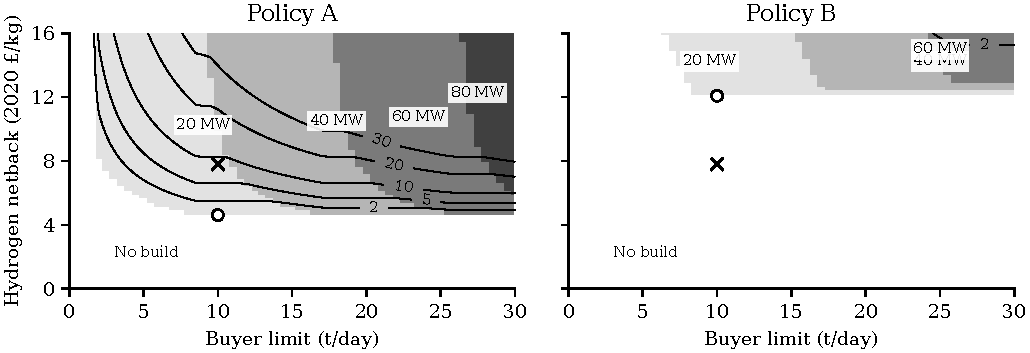
\includegraphics[width=\linewidth]{figures/contract_frontier.pdf}
\caption{2023 optimal capacity over 7,930 contract combinations. Contours
are annual gain (\gbp m); the cross marks the reference contract and the
circle the fixed 20 MW break-even at 10 t/day.}
\label{fig:contract}
\end{figure}

At 10 t/day, 20 MW breaks even at \gbp\BreakA/kg in A and
\gbp\BreakB/kg in B. At the reference netback, A first breaks even at
\OfftakeBreak~t/day. Table~\ref{tab:comparisons} shows why more equipment
needs a larger outlet: 40 MW reduces value at the original cap, while
50 t/day supports expansion in A but still no investment in B.

\begin{table}[H]
\centering\small
\caption{Sensitivity and operating comparisons (2023 unless marked). Electrolyser capacities $H_A,H_B$: MW; $v$: \gbp/kg; $L$ reported in t/day; capital: \gbp m; lost sales: GWh/year; gain: \gbp m/year. Capacity is optimised for sales floors/50 t, otherwise fixed; dashes mark A-only constraints.}
\label{tab:comparisons}
\begin{tabular}{@{}l r r r r r r r r@{}}
\toprule
Comparison & $H_A$ & $H_B$ & $v$ & $L$ & \shortstack{Capital\\A} & \shortstack{Lost\\sales A} & Gain A & Gain B \\
\midrule
Recover half of lost sales & 20 & -- & 7.80 & 10 & 29.2 & 79.0 & 5.19 & -- \\
Retain 99.99\% of sales & 20 & -- & 7.80 & 10 & 29.2 & 21.5 & 1.04 & -- \\
Fixed 40 MW & 40 & 40 & 7.80 & 10 & 58.4 & 183.9 & 7.47 & \minus{3.75} \\
50 t/day, free capacity & 120 & 0 & 7.80 & 50 & 175.3 & 923.6 & 49.09 & 0.00 \\
Capital +25\%, rate 8\% & 20 & 20 & 7.80 & 10 & 36.5 & 157.9 & 7.29 & \minus{2.35} \\
2025 downside & 20 & 20 & 4.00 & 5 & 29.2 & 49.2 & \minus{0.24} & \minus{0.77} \\
\bottomrule
\end{tabular}
\end{table}

Annual sales floors let the operator preserve selected electricity sales;
the 99.99\% floor binds, unlike a general statement that sales have priority.
The cost stress holds stack-renewal cost fixed; the joint 2025 downside
makes the fixed investment unprofitable under both policies.
The strict-quality 2023 subset keeps the original investment choices.

\subsection{Validation and conclusion}
The six-year battery revenue bound, even with free charging, is
\gbp\BatteryBound k per module-year in A, below the \gbp\BatteryCost k
annual cost. This rules out batteries in the common-size model. For one
fixed battery in 2023 A, replacing pooled energy with daily stock reduces
operating value from \gbp\PoolValue k to \gbp\StockValue k. The stock check
uses usable stock \(s_t=s_{t-1}+\eta c_t-r_t/\eta\),
\(0\le s_t\le E_Bb\), with zero initial and terminal stock.

All 60 exported Xpress schedules reconcile flow and cash, with physical
residuals below 0.001 MWh; eight contract points match exact enumeration.
All 14 annual replays agree with an independent implementation to its
published precision \cite{peer}. The 2023 A gain decomposes into
\gbp 23.97m hydrogen receipts, less \gbp 12.39m forgone electricity,
\gbp 0.52m fixed operation and \gbp 2.49m annual capital and stack cost.
Repeating that year's operating cash for 30 years gives a net present value
of \gbp\NPV m,
with simple/discounted paybacks of \Payback/\DiscountedPayback{} years,
including stack replacements and zero residual value.

Assess a 20 MW electrolyser against actual offtake and dispatch terms before
committing \gbp\Capital m, retaining B's loss-year risk. Zero battery
investment applies to the specified daily service and costs; intraday and
ancillary revenues are outside the model. Chapter~\ref{chap:tier2} examines
the chronology and restricted information absent from Tier 1.
